
% !TeX program = lualatex
% !TeX encoding = utf8
% !TeX spellcheck = uk_UA
% !BIB program = bibler

\documentclass{beamer}
\usetheme{Electromagnetism}
\usepackage{Electromagnetism}
\usetikzlibrary{spy}
\hypersetup{
  colorlinks=true,
  linkcolor=cyan,  % Цвет для внутренних ссылок
  urlcolor=red,    % Цвет для URL
  citecolor=blue   % Цвет для библиографических ссылок
}


%\def\colform#1{
%    \tikz[baseline]{\node[fill=green!50, rectangle, anchor=base, font=\scriptsize]{#1}}
%}


%============================================================================
\title[Лекції електрики та магнетизму]{\huge\bfseries Магнітне поле у речовині}
\subtitle{Лекції з електрики та магнетизму}
\author{Пономаренко С. М.}
\date{}
%============================================================================
\graphicspath{{pictures/}}

\begin{document}


\begin{frame}[plain]
	\maketitle
	%	\tikz[remember picture,overlay] \node[opacity=0.7,inner sep=0pt,
	%		anchor=north west] at (current page.north
	%	west){\includegraphics[width=2cm]{EMInteractions}};
\end{frame}

% ============================== Слайд ## ===================================
\begin{frame}{Зміст лекції}{}
	\tableofcontents
\end{frame}
% ===========================================================================


% ============================== Слайд ## ===================================
\begin{frame}{Гіпотеза Ампера}{Молекулярні струми}
	\begin{block}{}\justifying
		Якщо магнітне поле діє на рухомі заряджені частинки та рамки зі струмом, то \alert{чому воно також діє і на будь-який інший
			шматок магніту}? Ампер припустив, що \alert{всередині магніту теж течуть струми}.
	\end{block}


	\begin{block}{}\justifying\scriptsize
		Але якщо взяти стрілку або магніт у руки, то ніяких струмів ми не відчуваємо. Отже,  ці струми циркулюють усередині речовини і
		ніколи не виходять назовні. Що це за струми такі всередині речовини, Ампер звісно ж не знав. Сучасній науці вже відомо, що звичайна речовина
		складається з атомів. Своєю чергою, всередині атомів є позитивно заряджені ядра з негативно зарядженими електронами, що обертаються навколо них.
		Також самі електрони є маленькими магнітними стрілочками. Так
		ось, рух електронів усередині атомів є не що інше, як електричні струми, про існування яких припустив Ампер. Магнітне поле діє на ці струми, а
		значить і на речовину в цілому.
	\end{block}


	\begin{center}
		\includegraphics[width=1\linewidth]{AmpereHypotesis}
	\end{center}

\end{frame}
% ===========================================================================



% ============================== Слайд ## ===================================
\begin{frame}{Означення}{}
	\framesubtitle<1>{Мікрополе та середнє поле}
	\framesubtitle<2>{Струми провідності та молекулярні струми}
	\begin{onlyenv}<1>
		\begin{block}{}\justifying
			У речовині магнітне поле формується як зовнішнім полем, так і струмами, що циркулюють у цій речовині.

			\bigskip

			На мікрорівні (тобто на відстанях
			порядку розміру атомів і менше) поле різко змінюється в часі та просторі. Це поле називається \alert{мікрополем} $\Bfield_\text{micro}$ .
			Однак якщо провести усереднення за малим об'ємом, у якому є багато частинок (тобто за фізично нескінченно малим об'ємом), то отримаємо
			середнє поле:
			\begin{equation*}
				\left\langle \Bfield\right\rangle = \frac1{\Delta V} \iiint\limits_{\Delta V}
				\Bfield_\text{micro} dV.
			\end{equation*}
			\alert{Середнє поле} змінюється істотно повільніше внаслідок статистичного усереднення при випадковому русі частинок.
		\end{block}
	\end{onlyenv}
	\begin{onlyenv}<2>
		\begin{block}{}\justifying
			Створювані рухомими зарядами, можна розділити на дві групи: \alert{струми провідності} та \alert{молекулярні струми}.
			\begin{enumerate}
				\item \alert{Струми провідності} пов'язані з переміщенням вільних зарядів і є сторонніми щодо речовини.
				\item \alert{Молекулярні струми} зумовлені орбітальним рухом і спіном (власним моментом імпульсу) електронів в атомах (молекулах) і ядер речовини.
			\end{enumerate}
		\end{block}
	\end{onlyenv}
\end{frame}
% ===========================================================================


% ============================== Слайд ## ===================================
\begin{frame}{Вектор намагнічування}{}
	\begin{block}{}
		\alert{Вектор намагнічування} (або \alert{намагніченість}) — це величина, що характеризує магнітний момент одиниці об'єму речовини. Визначається вона
		як:

		\begin{equation*}
			\vect{J} = \frac{1}{V}\sum_i\vect{p}_i,
		\end{equation*}

		де $\vect{p}_i$ --- магнітні моменти окремих частинок.
	\end{block}


	\begin{block}{}\justifying\small
		Намагніченість називається \alert{однорідною}, якщо вектор $I$ не залежить від вибору точки в речовин. Якщо ж $\vect{I}\neq\const$, то намагніченість
		називається \alert{неоднорідною}.
	\end{block}
	\begin{center}
		\includegraphics[width=1\linewidth]{AmpereHypotesis}
	\end{center}
\end{frame}
% ===========================================================================


% ============================== Слайд ## ===================================
\begin{frame}{Вимірювані величини і вилучення струмів намагнічення}{}
	\begin{alertblock}{Основна задача теорії магнітостатики в речовині}\justifying
		У магнітостатиці стоїть завдання знайти спосіб опису полів, які виникають через молекулярні струми, без їх безпосереднього обчислення.
		Основна ідея полягає у тому, щоб \textbf{вилучити} струми намагнічення з рівнянь і замінити їх іншими величинами, які можливо вимірювати
		безпосередньо, наприклад, вектором намагнічення $\vec{J}$.
	\end{alertblock}
	\begin{block}{Чому це важливо?}\justifying
		Виключення струмів намагнічення з розрахунків дозволяє зосередитись на вимірюваних параметрах, що спрощує математичні моделі. В результаті,
		обчислення магнітних полів у магнетиках стає доступнішим і більш наочним.
	\end{block}
\end{frame}
% ===========================================================================


% ============================== Слайд ## ===================================
\begin{frame}{Зв'язок намагніченості з молекулярними струмами}{}


	\begin{block}{}\justifying\scriptsize
		Виділимо в речовині досить малий циліндр, так що поле в ньому можна вважати практично однорідним. У його об'ємі молекулярні струми компенсують один
		одного. Циліндр (ліворуч) і вигляд його торця (праворуч). Кільцеві струми, що циркулюють в об'ємі, компенсують один одного всюди, окрім точок бічної
		поверхні. У результаті залишається тільки поверхневий струм, що тече бічною поверхнею циліндра.
	\end{block}
	\begin{columns}
		\begin{column}{0.5\linewidth}\centering
			\begin{tikzpicture}[>=latex]
				\draw[fill=gray!20] (0,0) arc(180:350:1 and 0.2) -- ++(45:2)  arc(350:180:1 and 0.2) -- cycle;
				\path (45:2) ++(1,0) coordinate (O);

				\begin{scope}[shift={(O)}, yscale=0.2]
					\draw[thick, blue, arrowpos={0.7}{2pt}{3pt}] (0,0) [partial ellipse=0:360:1];
					\foreach \a in {10, 40,...,340} {
							\draw[red, smooth, arrowpos={0.75}{2pt}{3pt}] (\a:0.8) [partial ellipse=0:360:0.2];
						}
					\foreach \a in {25,85,...,335} {
							\draw[red, smooth] (\a:0.42) [partial ellipse=0:360:0.2];
						}
					\draw[red, smooth] (0, 0) [partial ellipse=0:360:0.2];
				\end{scope}

				\foreach \l in {0.2,0.4,...,1.8} {
						\draw[blue, arrowpos={0.4}{2pt}{3pt}] (45:\l) arc(180:350:1 and 0.2);
					}
				\draw[->, ultra thick] (O) -- ++(0,1) coordinate (J) node[left] {$\vect{J}$};
				\draw (0,0) -- ++(0,2);
				\draw (0,0) ++(0, 0.5) arc (90:45:0.5) node[pos=0.5, anchor=south] {$\theta$};
				\draw[->] (O) -- ++(45:{1*cos(45)}) coordinate (Pr) node[right] {$\ell\vect{\tau}$};
				\draw[dashed] (J) -- (Pr);
				\draw[<->] (2.2, 0) -- node[right] {$\ell$} ++(45:2);
			\end{tikzpicture}
		\end{column}
		\begin{column}{0.5\linewidth}\centering
			\begin{tikzpicture}[>=latex]
				\draw[arrowpos={0.4}{2pt}{4pt}, thick, blue] (0,0) [partial ellipse=0:360:1.01];
				\foreach \a in {10, 40,...,340} {
						\draw[arrowpos={\a/360}{2pt}{3pt}, red] (\a:0.8) [partial ellipse=0:360:0.2];
					}
				\foreach \a in {25,85,...,335} {
						\draw[arrowpos={\a/360}{2pt}{3pt}, red] (\a:0.42) [partial ellipse=0:360:0.2];
					}
				\draw[arrowpos={0.5}{2pt}{3pt}, red] (0, 0) [partial ellipse=0:360:0.2];
			\end{tikzpicture}
		\end{column}
	\end{columns}
	\begin{block}{}
		Знайдемо магнітний момент такого циліндрика:
		\begin{equation*}
			\vect{p}_m = \vect{J}V = \frac1c I_mS\ \vect{n} \Rightarrow\ \vect{J}S\ell\cos\theta = \frac1c I_m S\ \vect{n}
			\Rightarrow\ \vect{J}\cdot\vect{\ell} \ell\cos\theta  = \frac1c I_m \ \vect{n}\cdot\vect{\ell}
		\end{equation*}
		\begin{equation*}
			\frac{I_m}{\ell} = i_m = c\vect{J}\cdot\vect{\ell}.
		\end{equation*}
	\end{block}
\end{frame}
% ===========================================================================





% ============================== Слайд ## ===================================
\begin{frame}{Циркуляція вектора намагнічення}{}
	\framesubtitle<2>{Молекулярні об'ємні струми намагнічення}
	\begin{onlyenv}<1>
		\begin{columns}
			\begin{column}{0.5\linewidth}
				\begin{tikzpicture}[>=latex]
					\fill[red!20, draw=green!50!black, arrowpos={0.2}{0pt}{4pt}] (0,0) -- ++(4, 0) -- ++(-45:2) -- ++(-4, 0) --cycle;
					\foreach \x in {0,1,...,8}{
							\draw[arrowpos={0.45}{2pt}{3pt}, red, scale=0.5] (\x, 0) [partial ellipse=10:350:0.2 and 1];
							\draw[arrowpos={0.95}{2pt}{3pt}, red, scale=0.5] ({\x+3}, -2.8) [partial ellipse=10:350:0.12 and 0.6];
						}
					\draw[->, ultra thick, red!50, opacity=0.75] (2.8, -0.7) -- ++(0, -1.5) node[below] {$d\vect{S}$};
				\end{tikzpicture}
			\end{column}
			\begin{column}{0.5\linewidth}
				\begin{block}{}\justifying\small
					Виберемо тепер у речовині довільний замкнутий контур {\color{green!50!black}$L$}. На одиницю довжини контуру припадає струм
					намагнічування:
					\begin{equation*}
						i_m = c\vect{J}\cdot d\vect{\ell},
					\end{equation*}
					таким чином,  контур перетинає повний струм:
					\begin{equation*}
						I_m = c\oint\limits_L \vect{J}\cdot d\vect{\ell}.
					\end{equation*}
				\end{block}
			\end{column}
		\end{columns}
	\end{onlyenv}
	\begin{onlyenv}<1-2>
		\begin{block}{}\justifying
			Отриманий вираз на підставі теореми Стокса перетворюється на вигляд:
			\begin{equation*}
				I_m = c\oint\limits_L \vect{J}\cdot d\vect{\ell} = c \iint\limits_S \Rot\vect{J}\cdot d\vect{S}.
			\end{equation*}
			де $S$ --- поверхня, що спирається на контур $L$.
		\end{block}
	\end{onlyenv}
	\begin{onlyenv}<2>
		\begin{block}{}\justifying
			Струм, що протікає через поверхню $S$, виражається через густину струму формулою
			\(
			I_m = \iint\limits_S \vect{j}_m\cdot d\vect{S}.
			\)
			отже, що густина молекулярних струмів пов'язана з вектором намагнічування
			формулою:
			\begin{equation*}
				\tcbhighmath{\vect{j}_m = c\Rot\vect{J}.}
			\end{equation*}
			Це співвідношення дає \alert{зв'язок молекулярного струму з вектором намагнічування в диференціальній формі}.
		\end{block}
	\end{onlyenv}
\end{frame}
% ===========================================================================




% ============================== Слайд ## ===================================
\begin{frame}{Теорема про циркуляцію в речовині}{}
	\begin{onlyenv}<1>
		\begin{block}{}\justifying
			Циркуляцію магнітного поля породжують всі струми, як струми провідності так і струми намагнічування:
			\begin{equation*}
				\oint\limits_L\Bfield\cdot d\vect{\ell} = \frac{4\pi}c(I + I_m).
			\end{equation*}
			Тепер у нас є інструмент для вилучення $I_m$ з рівняння.
			\begin{equation*}
				\oint\limits_L\Bfield\cdot d\vect{\ell} = \frac{4\pi}c\left(I + c
				\iint\limits_S \Rot\vect{J}\cdot d\vect{S}\right).
			\end{equation*}
		\end{block}
	\end{onlyenv}
	\begin{onlyenv}<1-2>
		\begin{block}{}\justifying
			Введемо величину, що --- \alert{напруженість магнітного поля}:
			\begin{equation*}
				\tcbhighmath{\Hfield = \Bfield - 4\pi\vect{J}.}
			\end{equation*}
		\end{block}
	\end{onlyenv}
	\begin{onlyenv}<2>
		Теорема про циркуляцію в речовині прийме вигляд:
		\begin{columns}
			\begin{column}{0.5\linewidth}\centering
				\begin{equation*}
					\tcbhighmath{\oint\limits_L\Hfield\cdot d\vect{\ell} = \frac{4\pi}cI.}
				\end{equation*}
			\end{column}
			\begin{column}{0.5\linewidth}\centering
				\begin{equation*}
					\tcbhighmath{\Rot\Hfield = \frac{4\pi}c\vect{j}.}
				\end{equation*}
			\end{column}
		\end{columns}
		\begin{block}{}\justifying
			Вектор $\Hfield$ є допоміжним і слугує для спрощення вигляду рівнянь. Суттєво, що \alert{його циркуляція визначається тільки струмами провідності},
			що дає змогу в низці задач спростити розрахунок магнітного поля в середовищі.
		\end{block}
	\end{onlyenv}
\end{frame}
% ===========================================================================





% ============================== Слайд ## ===================================
\begin{frame}{Лінійні ізотропні магнітні середовища}{}
	\begin{block}{}
		Якщо магнітне поле слабке і в середовищі немає початкової намагніченості, то можна покласти:
		\begin{equation*}
			\vect{J} = \chi_m\Hfield.
		\end{equation*}
		Коефіцієнт $ \chi_m$ називається \alert{магнітною сприйнятливістю}.

		Підставимо це співвідношення у формулу $\Bfield = \Hfield + 4\pi\vect{J}$. Це дає
		\begin{equation*}
			\Bfield = (1+4\pi\chi_m)\Hfield = \mu\Hfield.
		\end{equation*}
		Величина $\tcbhighmath{\mu = 1+4\pi\chi_m}$ називається \alert{магнітною проникністю середовища}.
	\end{block}
\end{frame}
% ===========================================================================




% ============================== Слайд ## ===================================
\begin{frame}{Магнетики}{}\small
	\begin{block}{}\justifying
		Залежно від значення магнітної проникності виділяють такі основні класи середовищ:
		\begin{enumerate}
			\item Якщо $\chi_m > 0$, $\mu > 1$, то речовина називається \alert{парамагнетиком}. Парамагнітні властивості мають, наприклад,
			      \href{https://en.wikipedia.org/wiki/Aluminium}{\ce{Al}},
			      \href{https://en.wikipedia.org/wiki/Platinum}{\ce{Pt}},
			      \href{https://en.wikipedia.org/wiki/Iron(II)\_chloride}{\ce{FeCl2}},
			      \href{https://en.wikipedia.org/wiki/Oxygen}{\ce{O2}},
			      лужні та лужноземельні метали.

			\item Якщо $\chi_m < 0$, $\mu < 1$, то речовина називається \alert{діамагнетиком}. Діамагнетиками  є
			      \href{https://en.wikipedia.org/wiki/Bismuth}{\ce{Bi}},
			      \href{https://en.wikipedia.org/wiki/Antimony}{\ce{Sb}},
			      \href{https://en.wikipedia.org/wiki/Silicon}{\ce{Si}},
			      \href{https://en.wikipedia.org/wiki/Water}{\ce{H2O}},
			      \href{https://en.wikipedia.org/wiki/Dihydrogen}{\ce{H2}},
			      \href{https://en.wikipedia.org/wiki/Nitrogen}{\ce{N2}} тощо.
		\end{enumerate}
		Класифікація речовин на парамагнетики та діамагнетики запропонував М. Фарадей у 1845 р. Типові значення магнітної сприйнятливості для діа- і
		парамагнетиків становлять $|\mu| = 10^{-5} \div 10^{-5}$.
	\end{block}
	\vspace*{-1em}
	\begin{block}{}\justifying\footnotesize
		Деякі речовини можуть зберігати намагніченість $\vect{J}$ за відсутності зовнішнього магнітного поля. Для них не виконується просте співвідношення
		$\vect{J} = \chi_m\Hfield$ при всіх значеннях $\Hfield$. Такі речовини називаються \alert{феромагнетиками}. До їх числа належать, наприклад, \ce{Fe},
		\ce{Co}, \ce{Ni}. В діапазоні, де таке співвідношення формально виконується, магнітна проникність феромагнетиків сягає значень порядку $\mu
			\gg 1$.
	\end{block}
\end{frame}
% ===========================================================================





% ============================== Слайд ## ===================================
\begin{frame}{Граничні умови для $\Bfield$ та $\Hfield$}{}
	\begin{onlyenv}<1>
		\begin{columns}
			\begin{column}{0.6\linewidth}
				\begin{block}{}\scriptsize\justifying
					Застосуємо теорему Гауса до нескінченно малого циліндра, що охоплює частину межі
					розділу двох
					середовищ. Вважаючи $d\vect{S}_1 = - d\vect{S}_2$, $q = \sigma dS$,
					$d\vect{S}_1 =
						\vect{n}\ dS$,
					маємо
				\end{block}
			\end{column}
			\begin{column}{0.4\linewidth}\centering
				 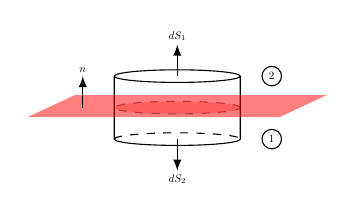
\begin{tikzpicture}[
scale=0.4,
transform shape,
>=latex,
declare function = {
h = 2;
r=2;
r2=0.2;
},
]

\fill[red!50, opacity=0.5, draw=black, dashed] (0,1) circle (r and r2);
\draw (-2,h) -- (-2,0) arc (180:360:r and r2) -- (2,h) ++ (-2,0) circle (r and r2);
\draw[dashed] (-2,0) arc (180:0:r and r2);
\fill[red,opacity=0.5]
 (-4.75,0.7) -- ++(8,0) -- ++(1.5,0.7) -- ++(-8,0) ;
\draw[->] (0,h) -- ++(0,1) node[above] {$d\vect{S}_1$};
\draw[->] (0,0) -- ++(0,-1) node[below] {$d\vect{S}_2$};

\draw[->] (-3,1) -- ++(0,1) node[above] {$\vect{n}$};

\node[circle, draw] at (3,0) {$1$};
\node[circle, draw] at (3,h) {$2$};
\end{tikzpicture}
			\end{column}
		\end{columns}
		\begin{block}{}\scriptsize
			\begin{equation*}
				\oiint_S \Bfield_1\cdot d\vect{S} = 0\ \Rightarrow  \Bfield_2\cdot
				d\vect{S}_1 +
				\Bfield\cdot d\vect{S}_2 = 0
			\end{equation*}
		\end{block}
		\begin{block}{}
			Звідси випливає перша гранична умова:
			\begin{equation*}
				\tcbhighmath{
					B_{1n} = B_{2n}.
				}
			\end{equation*}
		\end{block}
		\begin{alertblock}{}\justifying\scriptsize
			Нормальна складова вектора $\Bfield$ не зазнає стрибка при
			переході через границю розділу середовищ.
		\end{alertblock}
	\end{onlyenv}
	\begin{onlyenv}<2>
		\begin{columns}
			\begin{column}{0.6\linewidth}
				\begin{block}{}\scriptsize\justifying
					Застосуємо теорему про циркуляцію до нескінченно малого прямокутного
					контуру $L$, що проходить на нескінченно малій відстані над і під поверхнею
					розділу середовищ. Вважаючи, що $d\vect{r}_1 = -d\vect{r}_2$, маємо
				\end{block}
			\end{column}
			\begin{column}{0.4\linewidth}\centering
				 \begin{tikzpicture}[
scale=0.4,
transform shape,
>=latex,
declare function = {
h = 2;
r=2;
r2=0.2;
},
midarrow/.style={%
   postaction={ decorate,transform shape,
   decoration={ markings, mark=at position .5 with {\arrow{>}}}}},
]

\fill[red,opacity=0.5]
 (-4.75,0.7) -- ++(8,0) -- ++(1.5,0.7) -- ++(-8,0) ;

\draw[midarrow] (2, 1) -- ++(0, 1) -- node[above=5pt] {$L$} ++(-4, 0) -- ++(0, -1);
\draw[midarrow] (-2, 1) -- ++(0, -1) -- ++(4, 0) -- ++(0, 1);

\draw[->] (-3,1) -- ++(-2,0) node[above] {$\vect{\tau}$};
\draw[->] (-3,1) -- ++(0,1) node[above] {$\vect{n}$};
\draw[->] (-3,1) -- ++({180+45}:1) node[below] {$\vect{b}$};
\node[circle, draw] at (3,0) {$1$};
\node[circle, draw] at (3,h) {$2$};
\end{tikzpicture}
			\end{column}
		\end{columns}
		\begin{block}{}\scriptsize
			\begin{equation*}
				\oint\limits_L \Hfield\cdot d\vect{r} = \frac{4\pi}cI \Rightarrow \Hfield_1 d\vect{r}_1 +
				\Hfield_2 d\vect{r}_2 = \frac{4\pi}c i_b d\ell
			\end{equation*}
		\end{block}
		\begin{block}{}
			Звідси випливає друга гранична умова:
			\(
			\tcbhighmath{
				H_{2\tau} - H_{1\tau} = \frac{4\pi}c i_b.
			}
			\)
		\end{block}
		\begin{block}{}\justifying\scriptsize
			Останню умову можна можна записати у векторному вигляді: Оскільки $ \vect{\tau} = \vect{b}\times\vect{n} $. То $(\Hfield_2 - \Hfield_1)\vect{\tau} =
				\frac{4\pi}c i_b $, або $(\Hfield_2 - \Hfield_1)[\vect{b}\times\vect{n}] = \frac{4\pi}c i_b $. Зробивши циклічний зсув співмножників у змішаному
			добутку векторів, отримаємо:
			\(
				\tcbhighmath{
					\vect{n}\times (\Hfield_2 - \Hfield_1) = \frac{4\pi}c \vect{i}.
				}
			\)
		\end{block}
\begin{alertblock}{}\centering\scriptsize
    Тангенціальна складова $\Hfield$ зазнає розриву, якщо по поверхні розділу середовищ течуть \alert{струми провідності}.
\end{alertblock}
	\end{onlyenv}
\end{frame}
% ===========================================================================

\end{document}
